


%%%%%%%%%%%%%%%%
%%  Introduction
%%%%%%%%%%%%%%%%


%% Contents
%
%    - General considerations on Complex Systems, positioning etc (thesis in cs science etc)
%    - Thematic introduction, geographical introduction of the subject.
%
%   - precisions on v1 memoire : foreword ?
%
%    - reading precisions : organisation, interdependances etc 
%
%   - reflexive aspect : here ?  


%\chapter*{Introduction}{Introduction}
\chapter*{Introduction}


% to have header for non-numbered introduction
\markboth{Introduction}{Introduction}


% -- citations on hold --
%\headercit{\bpar{It's when you shuffle the anthill that you get a touch of all its complexity.}{C'est quand on donne un coup de pied dans la fourmilière qu'on se rend compte de toute sa complexité.\comment[AB]{je persiste a dire que c'est oas une tres bonne idee !}\comment[FL]{Incipit de son directeur de these est maladroit}}
%}{Arnaud Banos}{}



\bigskip




%\bpar{
%``In consequence of a technical issue, traffic is interrupted on the line B of RER, for an unknown duration. More information will be given as soon as available''. There is a high probability that someone having lived or spent some time in the metropolitan region of Paris has already heard this frightening announce and endured the difficult consequences the rest of his day. But he might not be aware of the ramifications of causal cascades induced by this not-so-rare event. Territorial Systems, whatever the layers considered in their definitions, will always be extremely complex and interrelations at numerous temporal and spatial scales participate in the emergent behaviors observed at any levels of the system. Martin is a student who daily commutes from Paris to Palaiseau and will miss today a crucial exam, what will have a profound impact on his professional life : implications at a long time scale, small spatial scale and agent granularity. Yuangsi is connecting Orly and Roissy Airports, in his trip from London to Beijing, will miss his plane and his sister's wedding : large spatial scale, short time scale, agent granularity. A collective petition emerges from users, leading to new social organizational patterns and reaction from transportation authority that results in efforts to increase levels of service : mesoscopic temporal and spatial scale, swarm of agents granularity. Looking for causes of the event will also lead to intricate processes at various scales, none of which seems to be a better explication than others : historical railway network in Parisian region shaped further extensions and RER B followed the former \textit{Ligne de Sceaux}, \noun{Delouvrier}'s schema for regional development, and its subsequent partial execution, are elements of explanation of structural weaknesses of Parisian public transportation network~\citep{gleyze2005vulnerabilite}; commuting patterns consequent to territorial organisation induce an overload of particular lines and thus a necessary increase in exploitation incidents. 
%}{
%``En conséquence d'un problème technique, le trafic est interrompu sur la ligne B du RER pour une durée indéterminée. Plus d'information seront fournies dès que possible''. Il y a des fortes chances pour que quiconque ayant vécu ou passé un peu de temps en région parisienne ait déjà entendu cette annonce glaçante et en ait subi les conséquences pour le reste de la journée. Mais il ne se doute sûrement pas des ramifications des cascades causales induites par cet évènement presque banal. Les systèmes territoriaux, quelles que soient les aspects considérés pour leur définition, ont une complexité croissante lorsqu'on augmente leur nombre, les interrelations à de nombreuses échelles spatiales et temporelles participant à la production des comportements émergents observés à tout niveau du système. Martin est un étudiant qui fait l'aller-retour journalier entre Paris et Palaiseau and manquera un examen crucial, ce qui aura un impact profond sur sa vie professionnelle : implications à une longue échelle de temps, une petite échelle spatiale et à la granularité de l'agent. Yuangxi était en train de relier les aéroports d'Orly et Roissy dans son voyage de Londres à Pékin et va manquer son avion ainsi que le mariage de sa soeur : grande échelle spatiale, courte échelle temporelle, granularité de l'agent. Une pétition collective émerge des voyageurs, conduisant à la création d'une organisation qui mettra la pression sur les autorités pour qu'elles augmentent le niveau de service : échelle temporelle et spatiales mesoscopique, granularité de l'aggregation d'agents.
%\comment[FL]{encore une fois : l'exemple mobilite quotidienne pour commencer me semble mal choisi}
%La recherche de cause possible à l'incident conduira à des processus intriqués à diverses échelles, parmi lesquels aucun ne semble être une meilleure explication ; le développement historique du réseau ferroviaire en région parisienne a conditionné les évolutions futures et le RER B a suivi l'ancienne Ligne de Sceaux, le plan de \noun{Delouvrier} pour le développement régional et son execution partielle, sont également des éléments d'explication de la structure du réseau parisien de transports en commun qui conditionne la perturbation~\cite{gleyze2005vulnerabilite} ; les motifs pendulaires dus à l'organisation territoriale induisent une surcharge de certaines ligne et ainsi nécessairement une augmentation des incidents d'exploitation.

%}


\bpar{}{
\textit{La machine à brouillard du Plateau de Saclay serait-elle le seul artefact intemporel dans cet environnement métropolitain qui se cherche toujours ? Projetons nous en 2100, dans cette banlieue sud parfois sordide de ce qui sera toujours Paris. Les bouleversements locaux ont bien eu lieu, mais pas de la façon attendue, le climat local étant toujours féru de ce fameux brouillard. Par contre, l'environnement urbain et la relation à la ville sont entièrement conditionnés par une grande proximité aux lignes de transport lourd : la disparition des moyens de transport thermiques, puis de l'ensemble des véhicules légers par échec technologiques des alternatives électriques, ont exacerbé le rôle des lignes de train ou de metro existantes. Les densités ont progressivement augmenté autour des gares pour produire d'impressionnants complexes de tours, tandis que les espaces péri-urbains se vidaient progressivement. Les infrastructures de transport sont quant à elles restées quasiment à l'identique après 2030, le peu de ressources disponibles étant dédié à leur entretien, et leur extension étant conjointement sortie rapidement des agendas politiques. Ce plateau est alors rempli de bâtiments à l'abandon, puisqu'il attend toujours ce tronçon du Grand Paris Express qui n'aura finalement jamais été réalisé. La nature reprend peu à peu ses droits.}
}


\bpar{}{
Ce pitch pour film d'anticipation à petit budget a pour avantage de nous révéler l'existence de processus complexes intriqués à différentes échelles de temps et d'espace dans la fabrique des villes : le développement historique du réseau ferroviaire en région parisienne a conditionné les évolutions futures et le RER B a suivi l'ancienne Ligne de Sceaux, le plan de \noun{Delouvrier} pour le développement régional et son execution partielle, sont des éléments d'explication de la structure du réseau parisien de transports en commun qui conditionne fortement le développement urbain dans notre scenario ; les processus de relocalisation au sein de l'espace de la métropole, liés à une plus ou moins grande nécessité de proximité ou d'accessibilité selon les modes de transports utilisés, participent à l'évolution urbaine ; dans le cas du plateau de Saclay des processus de planification spécifiques à différents niveaux jouent un rôle crucial dans la différentiation du territoire.
}



\bpar{
The list could be developed much longer and each approach related to an already mature scientific body of knowledge in different disciplines such as geography, urban economics, transportation. This amusing anecdote is enough to give a touch of the complexity of territorial systems. Our aim here is to dive into this complexity, and in particular to give an original insight into the study of relations between networks and territories. The choice of this reading position will be largely discussed in a further thematic part. Let for now concentrate on the originality of the point of view that we will take.
}{
La liste pourrait être ainsi continuée indéfiniment, chaque approche apportant sa vision mature correspondant à un corpus de connaissances scientifiques dans des disciplines diverses comme la géographie, l'économie urbaine, les transports. Cette anecdote est suffisante pour faire ressentir la complexité des systèmes territoriaux que nous étudierons. Notre but ici est de se plonger dans cette complexité, et en particulier donner un point de vue original sur l'étude des relations entre réseaux de transport et territoires. Le choix de cette position sera largement discuté dans une partie thématique, nous nous concentrons à présent sur l'originalité du point de vue que nous allons prendre.
}





\section*{On General Positioning}{De la position générale}


\bpar{
\emph{The ambition of this thesis is to have no ambition.} Such an introduction, although seeming rash, contains at all levels the implicit logics behind our research process. At the first degree, we try as much as possible to take a exploratory and constructive approach, as much on theoretical and methodological domains than thematic domain, but also proto-methodological (tools applying the method) : if unidimensional or integrated ambitions should emerge, they would be conditioned to the arbitrary choice of a time sampling among the continuity of the dynamic that structures any research project. In the structural sense, the self-reference that underlines an apparent contradiction points out the centra aspect of reflexivity in our constructive approach, as much in the sense of the recursion of theoretical apparels, than for application of tools and methods developed to the work itself, or in the sense of the co-construction of the different approaches and of the different thematic axis. The processus of knowledge production can this way be read as a metaphor of studied processes. Finally, from a point of view closer to interpretation, it suggests the intention of a delicate position linking a political positioning which necessity is intrinsic to humanities (for example here against the technocratic application of models, or for the development of tools for an Open Science) with a rigor of objectivity coming more from other fields used, position that impose an increased prudence.
}
{
\emph{L'ambition de cette thèse est de ne pas avoir d'ambition a priori.}
 Cette entrée en matière, rude en apparence, contient à différents niveaux les logiques sous-jacentes à notre processus de recherche. Au sens propre, nous nous plaçons tant que possible dans une démarche constructive et exploratoire, autant sur les plans théoriques et méthodologiques que thématique, mais encore proto-méthodologique (outils appliquant la méthode) : si des ambitions unidimensionnelles ou intégrées devaient émerger, elles seraient conditionnées par l'arbitraire choix d'un échantillon temporel parmi la continuité de la dynamique qui structure tout projet de recherche. Au sens structurel, l'auto-référence qui soulève une contradiction apparente met en exergue l'aspect central de la réflexivité dans notre démarche constructive, autant au sens de la récursivité des appareils théoriques, de celui de l'application des outils et méthodes développés au travail lui-même ou que de celui de la co-construction des différentes approches et des différents axes thématiques. Le processus de production de connaissance pourra ainsi être lu comme une métaphore des processus étudiés. Enfin, sur un plan plus enclin à l'interprétation, cela suggérera la volonté d'une position délicate liant une conscience politique dont la nécessité est intrinsèque aux sciences humaines (par exemple ici contre l'application technocratique des modèles, ou pour le développement d'outils luttant pour une science ouverte) à une rigueur d'objectivité plus propre aux autres champs abordés, position forçant à une prudence accrue.
}

%\comment[AB]{Déclaration discutable : si j’ai bien compris l’argumentaire, ton absence d’ambition tient 1) à l’absence de quête d’universalité (dépendance au contexte) et 2) à la dimension politique inhérente à ton objet. Je te ferais dire que 1) l’absence d’universalité n’est pas une tare (c’est même la norme en SHS) et 2) la dissociation science/politique ne tient plus la route depuis bien longtemps et ne concerne qu’un micro domaine des sciences les plus abstraites et théoriques (maths fondamentales, physique théorique peut-être,…what else ?)}[rq : logique proche de Morin - but contenu dans moyen ? - endogene.]



\section*{Scientific Context : Complexity Has Come of Age}{Contexte Scientifique : Paradigmes de la Complexité}


% \footnote{pour lesquels il n'existe pas de définition unifiée mais dont les champs d'application couvrent une étendue allant des neurosciences à la finance quantitative, en passant par exemple par la sociologie quantitative, la géographie quantitative, la biologie intégrative, etc.~\cite{newman2011complex}, et pour l'étude desquels diverses approches complémentaires peuvent être appliquées, comme les Systèmes Dynamiques, la Modélisation Basée Agent, la Théorie des Matrices Aléatoires}


\bpar{
To better introduce our subject, it is necessary to make the reader aware of the particular scientific context we are working in. It is necessary both to understand the general epistemology underlying research questions, and to be aware of the variety of methods and tools used. Contemporaneous science is progressively taking the shift of complexity in many fields.
That also implies an epistemological revolution to abandon strict reductionism that failed in most of its synthesis attempts~\cite{anderson1972more}. Arthur recently recalled~\cite{arthur2015complexity} that a mutation of methods and paradigms was also at stake by the increasing role of computational approaches replacing purely analytical techniques generally self-limited in their modeling and resolution scope. Capturing \emph{emergent properties} in models of complex systems is one of the ways to understand the essence of these new approaches.
}{
Pour une meilleure introduction du sujet, il est nécessaire d'insister sur le cadre scientifique dans lequel nous nous positionnons. Ce contexte est crucial à la fois pour comprendre les concepts épistémologiques implicites dans nos questions de recherche, et aussi pour être conscient de la variété de méthodes et outils utilisés. La science contemporaine prend progressivement le tournant de la complexité dans de nombreux champs que nous illustrerons par la suite, ce qui implique une mutation épistémologique pour abandonner le réductionnisme\footnote{De manière schématique, le réductionnisme consiste en la position épistémologique que les systèmes sont entièrement compréhensibles à partir des éléments fondamentaux les constituant et des lois régissant leur évolution. Les niveaux supérieurs n'ont ni autonomie ni pouvoirs causaux irréductibles.} strict qui a échoué dans la majorité de ses tentatives de synthèse~\cite{anderson1972more}. Arthur a rappelé récemment~\cite{arthur2015complexity} qu'une mutation des méthodes et paradigmes en était également un enjeu, de par la place grandissante prise par les approches computationnelles qui remplacent les résolutions purement analytiques généralement limitées en possibilités de modélisation et de résolution. La capture des \emph{propriétés émergentes} par des modèles de systèmes complexes est une des façons d'interpréter la philosophie de ces approaches.
}



\bpar{
These considerations are well known in Social Science (both quantitative and qualitative), in which the complexity of studied agents and systems is the justification of their existence : if humans were particles a whole branch of fields may have never emerged as thermodynamics would have solved most of social issues. \footnote{even if it would probably not have been the case as classical physics also failed in their attempts to include irreversibility and evolutions of Complex Adaptive Systems as Prigogine points out in \cite{prigogine1997end}} 
They are however less known nor accepted in more ``hard'' sciences such as physics : Laughlin develops in~\cite{laughlin2006different} a view of the discipline 
 at least as at a ``frontier of knowledge'' then other fields appearing as less mature. Most of knowledge is of classical nature although a majority of structures and systems would be \emph{self-organized}, what means that the single microscopic laws are not enough to determine macroscopic properties unless system evolution is simulated (more precisely this property can be taken as a definition of emergence on which we will come back further, and self-organization is intrinsically emergent). It corresponds to the first nightmare of Laplace's Deamon developed in~\cite{deffuant2015visions}.
}{
Ces considérations sont bien connues des Sciences Humaines et Sociales (qualitatives et quantitatives) pour lesquelles la complexité des agents et systèmes étudiés est une des justifications de leur existence : si les humains étaient effectivement des particules, on pourrait s'attendre à ce que la majorité des disciplines les prenant comme objet d'étude n'aient jamais émergé puisque la thermodynamique aurait alors résolu la majorité des problèmes sociaux\footnote{Bien que cette affirmation soit elle-même discutable, les sciences physiques classiques ayant également échoué à prendre en compte l'irréversibilité et l'évolution de Systèmes Complexes Adaptatifs comme le souligne~\cite{prigogine1997end}.}. Elles sont au contraire moins connues et acceptées en sciences ``dures'' comme la physique : \cite{laughlin2006different} développe une vision de la physique à la même position de ``frontière des connaissances'' que d'autre champs plus récents qui pourrait sembler en être encore à leur genèse. La plupart des connaissances actuelles concernent des structures classiques simples, alors qu'un grand nombre de systèmes présentent des propriétés \emph{d'auto-organisation}, au sens où les lois microscopiques ne sont pas suffisantes pour inférer les propriétés macroscopiques du système à moins que son évolution ne soit entièrement simulée (plus précisément cette vision peut être prise comme une définition de l'émergence sur laquelle nous reviendrons par la suite, or des propriétés auto-organisées sont par nature émergentes). Cela correspond au premier cauchemar du Démon de Laplace développé dans~\cite{deffuant2015visions}. 
} 


%-------------------------------------------------



\bpar{
As an informal mix of epistemological positions, methods, and fields of applications, \emph{Complexity Science} relies on typical paradigms such as the centrality of emergence and self-organization in most of phenomena of the real world, which make it lie on a frontier of knowledge closer of us than we can think (Laughlin, op.cit. ). Such concepts are indeed not new, as they were already enlighten by Anderson~\cite{anderson1972more}. Even cybernetics can be related to complexity by seing it as a bridge between technology and cognitive science~\cite{wiener1948cybernetics}.
}{
A la croisée de positionnements épistémologiques, de méthodes et de champs d'application, les \emph{Sciences de la complexité} se concentrent sur l'importance de l'émergence et de l'auto-organisation dans la plupart des phénomènes réel, ce qui les place plus proche de la frontière des connaissances que ce que l'on peut penser pour des disciplines classiques (\noun{Laughlin}, op. cit.). Ces concepts ne sont pas récents et avaient déjà été mis en valeur par~\cite{anderson1972more}. On peut aussi interpréter la Cybernétique comme un précurseur des Sciences de la Complexité en la lisant comme un pont entre technologie et sciences cognitives~\cite{wiener1948cybernetics}, et surtout en développant les notions de retroaction et de contrôle.
}

\bpar{
Later, synergetics~\cite{haken1980synergetics} paved the way for a theoretical approach of collective phenomena in physics. Reasons for the recent growth of works claiming a CS approach may be various. The explosion of computing power is surely one because of the central role of numerical simulations~\cite{varenne2010simulations}. They could also be the related epistemological progresses : apparition of the notion of perspectivism~\cite{giere2010scientific}, finer reflexions around the notion of model~\cite{varenne2013modeliser}\footnote{In that frame scientific and epistemological progress can not be dissociated and can be seen as coevolving}. The theoretical and empirical potentialities of such approaches play surely a role in their success\footnote{
Although the adoption of new scientific practices may be strongly biased by imitation and lack of originality~\cite{dirk1999measure}, or more ambivalent, by marketing strategies as the fight for funds is becoming a huge obstacle for research~\cite{bollen2014funding}.}, as confirmed in various domains of application (see~\cite{newman2011complex} for a general survey), as for example Network Science~\cite{barabasi2002linked} ; Neuroscience~\cite{koch1999complexity}; Social Sciences ; Geography~\cite{manson2001simplifying}\cite{pumain1997pour} ; Finance with the rising importance of econophysics~\cite{stanley1999econophysics} ; Ecology~\cite{grimm2005pattern}. The Complex Systems Roadmap~\cite{2009arXiv0907.2221B} proposed a double lecture of studies on Complex Systems : an horizontal approach connecting fields of study with transversal questions on theoretical foundations of complexity and empirical common stylized facts, and a vertical conceptions of disciplines, with the aim to construct integrated disciplines and corresponding multi-scale heterogeneous models. Interdisciplinarity is thus central in our scientific background.
}{
Plus tard, la Synergétique~\cite{haken1980synergetics} a posé les bases d'approches théoriques des phénomènes collectifs en physique. Les causes possibles de la croissance récente du nombre de travaux se réclamant d'approches complexes sont nombreuses. L'explosion de la puissance de calcul en est certainement une vu le rôle central que jouent les simulations numériques~\cite{varenne2010simulations}. Elles peuvent aussi être à chercher auprès de progrès en épistémologie : introduction de la notion de perspectivisme~\cite{giere2010scientific}, reflexions plus fine autour de la nature des modèles~\cite{varenne2013modeliser}\footnote{Dans ce cadre, les progrès scientifiques et épistémologiques ne peuvent pas être dissociés et peuvent être vus comme étant en co-évolution, au sens d'une forte interdépendance et d'une adaptation mutuelle.}. Les potentialités théoriques et empiriques de telles approchent jouent nécessairement un rôle dans leur succès\footnote{Même si l'adoption de nouvelles pratiques scientifiques peut par ailleurs être biaisé par l'imitation et le manque d'originalité~\cite{dirk1999measure}, ou de façon plus ambivalente, par des stratégies de positionnement indépendante des stratégies de connaissance, puisque le combat pour les fonds est un obstacle croissant à une recherche saine~\cite{bollen2014funding}.}, comme le confirme les domaines très variés d'application (voir~\cite{newman2011complex} pour une revue très générale), comme par exemple la Science de Réseaux~\cite{barabasi2002linked}; les Neurosciences~\cite{koch1999complexity}; les Sciences Humaines et Sociales,  dont la Géographie~\cite{manson2001simplifying}\cite{pumain1997pour}; la Finance avec les approches écononophysiques~\cite{stanley1999econophysics}; l'Ecologie~\cite{grimm2005pattern}. La Feuille de Route des Systèmes Complexes~\cite{2009arXiv0907.2221B} propose une double lecture des travaux en Complexité: une approche horizontale faisant la connexion entre champs d'étude par des questions transversales sur les fondations théoriques de la complexité et des faits stylisés empiriques communs, et une approche verticale, dans le but de construire des disciplines intégrées et les modèles multi-scalaires hétérogènes correspondants. L'interdisciplinarité est ainsi cruciale pour notre contexte scientifique.

}


\section*{Interdisciplinarity}{Interdisciplinarité}

%\comment[FL]{pkoi pas dans ch3 ?}[on en a deja parlé pas mal, pour moi c'est essentiel de poser le cadre general et l'ambiance en intro]

\bpar{
We must further insist on the role of interdisciplinarity in the positions taken here. This is not a thesis in Geography nor in Complex Adaptive Systems Modeling,
 but in \emph{Complex Systems Science} that we claim as a proper discipline following \noun{Paul Bourgine}.
  It will naturally be seen with defiance by scholars of various concerned disciplines, as recent examples of misunderstandings and conflicts have illustrated~\cite{dupuy2015sciences}.
}{
Il est important d'insister sur le rôle de l'interdisciplinarité dans la position de recherche prise ici. Il s'agit autant d'un travail en Géographie Théorique et Quantitative qu'en Modélisation de Systèmes Complexes, étant finalement les deux à la fois selon le point de vue que prendra le lecteur. En ce sens, nous le réclamons de la \emph{Science des Systèmes Complexes} que nous tenterons de positionner comme discipline propre à travers cette implémentation précise\footnote{Un niveau de lecture abstrait du travail dans son ensemble apportera des informations sur la production de connaissance elle-même, comme nous le développerons en~\ref{sec:knowledgeframework}.}. Ce n'est pas sans risques d'être lu avec méfiance voir défiance par les tenants des disciplines classiques, comme des exemples récents de malentendus ou conflits ont récemment illustré~\cite{dupuy2015sciences}. Il faut se rappeler l'importance de la spirale vertueuse de \noun{Banos} entre disciplinarité et interdisciplinarité~\cite{banos2013pour}. Celle-ci doit nécessairement impliquer différents agents scientifiques, et il est compliqué pour un agent de se positionner dans les deux branches ; notre fond scientifique devra nous permettre de ne pas de nous positionner uniquement dans la \emph{disciplinarité géographique} (même si celle-ci sera simultanément une composante cruciale) mais bien aussi dans celle des Systèmes Complexes (qui est interdisciplinaire, voir~\ref{sec:epistemology} pour contourner la contradiction apparente), et notre sensibilité scientifique et épistémologique nous pousse à faire de même.
}

% rq : point de vue = grille de lecture
% \comment[AB]{je trouve que tu abandonnes bien vite la partie. Pourquoi renoncer dès le début alors que tu pourrais laisser la liberté à celui/celle qui te lit de décider si c’est AUSSI de la géo ou non ?}


% -- inutile --
%\bpar{
%The positioning of \noun{Batty} proposing \textit{A new Science of Cities}~\cite{batty2013new} (that he subtly presents as \textit{The} new science of cities) is directed towards an integration of disciplines and methods into a science defined by its object of study, cities.
%Its theoretical and epistemological weaknesses (no theoretical constructions of studied geographical objects on the one hand, approximative contextualization of complexity) combined with an overall impression of \emph{pot-pourri} of forgotten works
% (space syntax, land-use models), unfortunately avoid us to use it as we will use geographical theories (e.g. evolutive urban theory) in an appropriated epistemological complexity context. Yet our reading of this work may be the result of a misunderstanding due to different cultural backgrounds.
%}
%{
%Le positionnement de \noun{Batty} lorsqu'il propose \textit{Une Nouvelle Science des Villes}~\cite{batty2013new} %(qu'il présente avec humour comme \textit{La} nouvelle science des villes)
%, se présente comme une intégration des disciplines et méthodes vers une science définie par son objet d'étude, les villes.
%Its theoretical and epistemological weaknesses (no theoretical constructions of studied geographical objects on the one hand, approximative contextualization of complexity) combined with an overall impression of \emph{pot-pourri} of forgotten works (space syntax, land-use models), unfortunately avoid us to use it as we will use geographical theories (e.g. evolutive urban theory) in an appropriated epistemological complexity context.  Yet our reading of this work may be the result of a misunderstanding due to different cultural backgrounds. \comment[Arnaud]{j'espère que tu abuses ? :) !! Argument d'autorité}[yes, changer positionnement complètement malvenu] \comment[Florent]{attention arguments autorité ; insister sur difficulté à intégrer paradigmes plutot que juger précédents}[idem]
%}




\bpar{
The scientific evolution of complexity that some see as a revolution~\cite{colander2003complexity}, or even as \emph{a new kind of science}~\cite{wolfram2002new}, could indeed face intrinsic difficulties due to behaviors and a-priori of researchers as human beings.
 More precisely, the need of interdisciplinarity that makes the strength of Complexity Science may be one of its greatest weaknesses, since the highly partitioned structure of science organization has sometimes negative impacts on works involving different disciplines. We do not tackle the issue of over-publication, competition, indexes, which is more linked to a question of open science and its ethics, also of high importance but of an other nature. That barrier we are dealing with and we might struggle to triumph of, is the impact of certains \emph{cultural disciplinary differences} and out-coming conflicts on views and approaches. 
The drama of scientific misunderstandings is that they can indeed annihilate progresses by interpreting as a falsification some work that answers to a totally different question. The example of a recent work on top-income inequalities given in~\cite{aghion2015innovation}, which conclusions are presented as opposed from the one obtained by Piketty~\cite{piketty2013capital}, follows such a scheme. Whereas Piketty focused on constructing long-time clean databases for income data and showed empirically a recent acceleration of income inequalities, his simple model aiming to link this stylized fact with the accumulation of capital has been criticized as oversimplified. On the other hand, Bergeaud \textit{et al.} prove by a model of innovation economics that \emph{under certain assumptions} income gaps may be beneficial to innovation and consequently a general utility. Thus diverging conclusions about the role of personal capitals in the economy.
But diverging \emph{views} or \emph{interpretations} does not mean a scientific incompatibility, and one could imagine try to gather both approaches in an unified framework and model, yielding possibly similar or different interpretations. This integrated approach has chances to contain more information (depending on how coupling is done) and to be a further advance in Science. In an other but similar vein, \cite{2017arXiv170105627H} reanalyses biological data from a 1943 experiment that claimed to rule out Lamarckian over Darwinian evolution processes, and show that the conclusion are wrong in the current Data analysis (enormous advances in theoretical and processing techniques) and scientific context (with numerous other proofs today of Darwinian processes) : this is a good example of a context-misunderstanding and how conclusions strongly depend on both technical and thematic frameworks. We shall now briefly develop other examples to give an overview how conflicts between disciplines can be damaging.
}{
L'évolution scientifique des sciences de la complexité, qui est vue par certains comme une révolution~\cite{colander2003complexity}, ou même comme \emph{un nouveau type de science}~\cite{wolfram2002new}, pourrait affronter des difficultés intrinsèques dues aux comportements et a-priori des chercheurs en tant qu'être humains. Plus précisément, le besoin d'interdisciplinarité qui fait la force des Sciences de la Complexité pourrait devenir une de ses grandes faiblesses, puisque la structure fortement en silo de la science peut avoir des impacts négatifs sur les initiatives impliquant des disciplines variées. Nous n'évoquons pas les problèmes de sur-publication, quantification, competition, qui sont plus liés à des questions de Science Ouverte et de son éthique, tout aussi de grande importance mais d'une autre nature. Cette barrière qui nous hante et que nous pourrions ne pas surmonter, a pour plus évident symptôme des \emph{divergences culturelles disciplinaires}, et les conflits d'opinion en résultant. Ce drame du malentendu scientifique est d'autant plus grave qu'il peut en effet détruire totalement certains progrès en interprétant comme une falsification des travaux qui traitent une question toute différente. L'exemple récent en économie d'un travail sur les inégalités liées aux hauts revenus présenté dans~\cite{aghion2015innovation}, et dont les conclusions ont été commentées comme s'opposant aux thèses de~\cite{piketty2013capital}, est typique de ce schéma. Ce second se concentre sur la construction de bases de données propres sur le temps long pour les revenus et montre empiriquement une récente accélération des inégalités de revenus, son modèle visant à lier ce fait stylisé avec l'accumulation de capital a été critiqué comme trop simpliste. D'autre part, \cite{aghion2015innovation} montrent par des analyses économétriques que s'il existe bien un lien de causalité de l'innovation vers les inégalités de haut salaires, l'innovation accroit cependant la mobilité sociale, étant donc également moteur de réduction des inégalités. D'où des conclusions divergentes sur le rôles des capitaux personnels dans une économie, notamment sur leur relation ambigüe à l'innovation. Mais des \emph{point de vue} ou \emph{interprétations} différentes ne signifient pas une incompatibilité scientifique, et on pourrait même imaginer rassembler ces deux approches dans un cadre et modèle unifié, produisant des interprétations possiblement similaires et potentiellement encore nouvelles. Une telle approche intégrée aura de grandes chances de contenir plus d'information (selon la façon dont le couplage est opéré) et être une avancée scientifique. Cette expérience de pensée illustre les potentialités et la nécessité de l'interdisciplinarité. Dans une autre veine assez similaire, \cite{2017arXiv170105627H} ré-analyse des données biologiques d'une expérience de 1943 qui prétendait confirmer l'hypothèse des processus d'évolution Darwiniens par rapport aux processus Lamarckiens, et montrent que les conclusions ne tiennent plus dans le contexte actuel d'analyse de données (avances énormes sur la théorie et les possibilités de traitement) et scientifique (avec d'autres nombreuses preuves de nos jours des processus Darwiniens) : c'est un bon exemple de malentendu sur le contexte, et la manière selon laquelle le cadre de travail à la fois technique et thématique influence fortement les conclusions scientifiques. Nous développons à présent divers exemples révélateurs de la manière dont des conflits entre disciplines peuvent être dommageables.
}

%\comment[AB]{tout ceci remet en question ton « absence d’ambition » me semble-t-il}[par l'amplitude disciplinaire recherchée tu veux dire ?]

%\paragraph{Physics reinvents geography}{La tentation de réinventer la géographie}


\bpar{
As already mentioned, \noun{Dupuy} and \noun{Benguigui} points out in \cite{dupuy2015sciences} the fact that urban sciences
 have recently known open conflicts between old tenants of the disciplines and new arrivants, especially physicists.
 The availability of large datasets of new type of data (social networks, ICT data) have drawn their attention towards the study of objects traditionally studied by human science, as analytical and computational methods of statistical physics became applicable. Although these studies are generally presented as the construction of a scientific approach to cities, implying that existing knowledge was not scientific because of their more qualitative aspect, they have not unveil specifically novel knowledge on urban systems : 
  to give some examples, \cite{barthelemy2013self} concludes that Paris has followed a transition during Haussman period and that the evolution of a city is the combination of local transformations and global planning operations, what are facts known for a long time in urban history and urban geography. \comment{(Florent) qui a découvert avant ?}
  \cite{chen2009urban} rediscovers that the gravity model can be improved by adding lags in interactions and theoretically derives the expression of the force of interaction between cities, without any thematic theoretical background. Examples could be multiplied, confirming the current discomfort in communication between physicists and urban geographers. Significant benefices could results from a wise integration of disciplines~\cite{o2015physicists} but the road seems still long. 
}{
Comme déjà mentionné, \noun{Dupuy} et \noun{Benguigui} soulignent dans~\cite{dupuy2015sciences} le fait que dans le domaine de l'urbanisme, ont récemment éclaté des conflits ouverts entre les tenants classiques des disciplines et des nouveaux arrivants, en particulier les physiciens, même si leur entrée dans le domaine n'est pas nouvelle. La disponibilité de grand jeux de données d'un nouveau type (réseaux sociaux, données des nouvelles technologies de la communication) ont attiré l'attention d'un plus grand nombre sur des objets plus traditionnellement étudiés par les sciences humaines, puisque les méthodes analytiques et computationnelles de la physique statistique sont devenues applicables. Bien que ces travaux soient généralement présentés comme la construction d'une approche scientifique des villes, tout en discutant la nature scientifique des approches existantes, la nouveauté réelle des résultats obtenus et la non-légitimation des approches ``classiques'' sont discutables. Pour citer quelques exemples, \cite{barthelemy2013self} conclut que Paris a subit une transition pendant la période d'Haussman et ses opérations de planification globale, qui sont des faits naturellement connus depuis longtemps en Histoire Urbaine et Géographie Urbaine. \cite{chen2009urban} redécouvre que le modèle gravitaire est amélioré par l'introduction de décalages dans les interactions et dérive analytiquement l'expression d'une force d'interaction entre les villes, sans se placer dans un cadre théorique ou thématique. De tels exemples peuvent être multipliés, confirmant l'inconfort courant entre physiciens et géographes. Des bénéfices significatifs pourraient résulter d'une intégration raisonnée des disciplines~\cite{o2015physicists} mais la route semble être bien longue encore.
}


%\paragraph{Economic Geography or Geographical Economics ?}{Economie Géographie ou Géographie Economique ?}


\bpar{
Similar conflict occurred in economics : as \cite{marchionni2004geographical} describes, the discipline of economic geography, traditionally close from geography, heavily criticized a new stream of thought named \emph{geographical economics}, which purposes is spatialization of mainstream economic techniques. Both do not have the same purposes and aims, and the conflict appears as a total misunderstanding for an external observer.
}{
Des conflits similaires se rencontrent à l'interface des relations entre économie et géographie : comme le décrit \cite{marchionni2004geographical}, la discipline de la géographique économique, traditionnellement proche de la géographie, a fortement critiqué à son émergence l'approche relativement récente \emph{Nouvelle Economie Géographique}. Celle-ci provient de l'économie et son but est la prise en compte de l'espace par les méthodes économiques classiques. Elles n'ont en fait pas les mêmes desseins et buts, et le conflit apparaît comme un malentendu complet vu d'un oeil extérieur. Par exemple, la Nouvelle Economie Géographique privilégiera des explications impliquant des processus économiques universels et indépendant des échelles, tandis que la Géographie Economique basera son argumentation sur les particularité locales et la contingence des processus. Les hypothèses épistémologiques sous-jacentes sont également très différentes, comme par exemple la relation au réalisme, la première étant fondée sur un réalisme abstrait pas forcément concrètement réaliste (utilisation de processus abstraits), tandis que la deuxième sera plus pragmatique. La mesure dans laquelle ces deux approches sont complémentaires ou incompatible reste toutefois une question ouverte d'après \cite{marchionni2004geographical}. Des relations disciplinaires similaires seront rencontrées dans notre travail, comme entre la physique et la géographie. Nous développons par ailleurs en~\ref{app:sec:ecogeo} une exploration des liens entre économie et  géographie du point de vue de la modélisation.
}



%\paragraph{Agent-based Modeling in Economy}{Modélisation basée agent en Economie}


\bpar{
Disciplinary conflicts may also manifest themselves as the reject of novel methods by mainstream currents. Following \cite{farmer2009economy}, the operational failure of most classic economic approaches could be compensated by a broader use of agent-based modeling and simulation practices. The lack of analytical framework that is natural in the study of complex adaptive systems seems to be rebutting for most of economists.
}{
Des conflits disciplinaires peuvent aussi se manifester sous la forme d'un rejet de méthodes nouvelles par les courants dominants. Suivant \noun{Farmer}~\cite{farmer2009economy}, l'échec opérationnel de la plupart des approches économiques classiques pourrait être compensé par un usage plus systématique de la modélisation et simulation basées agent. L'absence de résolution analytique qui est inévitable pour l'étude de la plupart des systèmes complexes adaptatifs semble rebuter la plupart des économistes. Or, \cite{barthelemy2016structure} insiste sur la déconnexion exacerbée entre une grande partie des modèles et théories économiques et les observations empiriques, du moins dans le domaine de l'économie urbaine. Celle-ci pourrait être un symptôme de la déconnexion disciplinaire évoquée ci-dessus. Toujours en économie, \cite{storper2009rethinking} propose aussi des changements de paradigmes par un retour à l'agent et une construction associée de théories \emph{evidence-based}.
}


%\paragraph{Finance}{Finance}

\bpar{
In Quantitative Finance coexist various stream of research with a very few interactions. Let consider two examples. On the one hand, Statistics are highly advanced in theoretical mathematics, using stochastic calculus and probabilities to obtain very refined estimators of parameters for a given model (see e.g. \cite{barndorff2011multivariate}). On the other hand, Econophysics aims to study empirical stylized facts and infer empirical laws to explain complexity-related phenomena in financial systems~\cite{stanley1999econophysics}, such as e.g. cascades leading to market crashes, fractal properties of asset signals, complex structure of correlation networks. Both have their advantages in a particular context and each would benefit from increased interactions between the fields.
}{
La finance quantitative peut être instructive pour notre propos et sujet, d'une part par les similarités de la cuisine interdisciplinaire avec notre domaine (rapport avec la physique et l'économie, champs plus ou moins ``rigoureux'', etc.). Dans ce domaine coexistent divers champs de recherche ayant très peu d'interactions entre eux. On peut considérer deux exemples. D'une part, les statistiques et l'économétrie sont extrêmement avancées en mathématiques théoriques, utilisant par exemple des méthodes de calcul stochastique et de théorie des probabilité pour obtenir des estimateurs très raffinés de paramètres pour un modèle donné (voir par exemple \cite{barndorff2011multivariate}). D'autre part, l'éconophysique a pour but d'étudier des faits stylisés empiriques et inférer les lois correspondantes pour tenter d'expliquer des phénomènes économiques, par exemple ceux liés à la complexité des marchés financiers~\cite{stanley1999econophysics}. Ceux-ci incluent les cascades menant aux ruptures de marché, les propriétés fractales des signaux des actifs, la structure complexe des réseaux de corrélation. Chacun a ses avantages dans un contexte particulier et gagnerait à des interactions accrues entre les deux domaines.
}


\bpar{
These diverse examples illustrate how interdisciplinarity is both crucial and difficult to achieve. We will try to follow that narrow path in our work, borrowing ideas, theories and methods from various disciplines, aiming for the construction of an integrated knowledge. Indeed, coupling heterogeneous approaches at different levels and scales 
will be a cornerstone of our thesis, skeleton of the underlying philosophy and building brick of the theory we will propose.
}{
Ces divers exemples pris au fil du vent sont de brèves illustrations du caractère crucial de l'interdisciplinarité et de sa difficulté à pratiquer. Sans presque exagérer, on pourrait imaginer l'ensemble des chercheurs se plaindre de mauvaises ou difficiles expériences d'interdisciplinarité, avec un retour largement positif lors des rares succès. Nous allons tenter par la suite d'emprunter ce chemin étroit, empruntant des idées, théories et méthodes de diverse disciplines, dans l'idéal de la construction d'une connaissance intégrée.
}


%\comment[JR]{également un développement sur ``quanti-quali'' ?}
% pas besoin : en ouverture avec domaines connaissance a la fin.






%-------------------------------------------------

\section*{Complexity in Geography}{Paradigmes de la Complexité en Géographie}

%\comment[FL]{idem}[idem]

\bpar{
Coming back to our introducing anecdote, we will focus on our thematic object of study that are territorial systems.
 More generally, we propose an overview of the role of complexity in geography. Geographers are familiar with complexity for a long time, as the study of spatial interactions is one of its purposes. The variety of fields in geography (geomorphology, physical geography, environmental geography, human geography, health geography to give a few) has certainly been important in the subtlety of the geographical thinking, that considers heterogeneous and multi-scalar processes.
}{
Pour revenir à notre anecdote introductive, nous nous concentrons sur l'étude d'un objet thématique qui sera les systèmes territoriaux : à l'échelle microscopique, les agents peuvent bien être vus comme éléments constitutifs fondamentaux du territoire, qui émergera comme processus complexe à différentes échelles. Plus généralement, il s'agit par commencer de brosser une revue du rôle de la complexité en géographie. Les géographes sont naturellement familiers avec la complexité, puisque l'étude des interactions spatiales est l'un de leurs objets de prédilection. La variété de champs en géographie (géomorphologie, géographie physique, géographie environnementale, géographie humaine, géographie de la santé, etc. pour en nommer certains) a sûrement joué un rôle clé dans la constitution d'une pensée géographique subtile, qui considère des processus hétérogènes et multi-scalaires.
}



\bpar{
\noun{Pumain} recalls in~\cite{pumain2003approche} a subjective history of the emergence of complexity paradigms in geography. Cybernetics yielded system theories as the one developed by Forrester.
 Later the shift to self-organized criticality and self-organisation concepts in physics conducted to corresponding developments in geography, as \cite{sanders1992systeme} witnesses the application of the concepts of synergetics for the dynamics of an urban system.
}{
\noun{Pumain} rappelle dans~\cite{pumain2003approche} une histoire subjective de l'émergence des paradigmes de la complexité en géographie, que nous restituons ici. La cybernétique a produit des théories des systèmes comme celle utilisée pour les premiers modèles de dynamique des systèmes visant à simuler l'évolution de variables caractérisant un territoire, sous la forme d'équations différentielles couplées, comme \cite{chamussy1984dynamique} l'illustre pour un modèle couplant population, emplois et stock de logements. Plus tard, le glissement vers les concepts de criticalité auto-organisée et d'auto-organisation en physique ont conduit aux développements correspondants en géographie, comme~\cite{sanders1992systeme} qui témoigne de l'application des concepts de la synergétique aux dynamiques des systèmes urbains.
}


\bpar{
Finally, Complex Systems paradigms as we currently know them appeared from various points of view.
}{
Enfin, les paradigmes actuels des systèmes complexes ont été introduits par plusieurs entrées relativement indépendantes. On peut nommer parmi celles-ci les concepts issus des fractales, les automates cellulaires, le \emph{Scaling}, et la Théorie Evolutive des Villes. Nous revoyons brièvement ces approches ci-dessous.
}


\bpar{
The fractal nature of urban shape was introduced in~\cite{batty1994fractal} and had numerous application including more recent developments~\cite{keersmaecker2003using}.
}{
L'étude de la nature fractale de la forme urbaine a été introduite par~\cite{batty1986fractal}, plus tard synthétisée par~\cite{batty1994fractal} et a eu de nombreuses applications jusqu'à des développements plus récents comme~\cite{keersmaecker2003using} pour l'analyse de la forme urbaine ou~\cite{tannier:hal-00860260} pour l'élaboration de planifications urbaines durables.
}

%\comment{lier avec les approches de Frankhauser citer  http://www.persee.fr/doc/spgeo\_0046-2497\_1990\_num\_19\_1\_2943 ?}

\bpar{
}{
La Théorie du \emph{Scaling} a par ailleurs été importée de la physique et de la biologie et des relations allométriques pour expliquer les lois d'échelle urbaine comme propriétés universelles liées au type d'activité : infrastructure et économies d'agglomération (scaling infralinéaire) ou résultante d'un processus d'interactions sociales (scaling supralinéaire), et suppose les villes comme versions à l'échelle l'une de l'autre~\cite{bettencourt2007growth}. Nous n'utiliserons pas explicitement ces deux approches mais celles-ci restent sous-jacentes dans les paradigmes utilisés\footnote{Par exemple, les lois d'échelles ont une place privilégiée dans l'application de la Théorie Evolutive~\cite{pumain2006evolutionary}.}.
}



\bpar{
\noun{Batty} also introduced cellular automata in urban modeling and proposed a joint synthesis with agent-based modeling and fractals in~\cite{batty2007cities}.
}{
Les automates cellulaires, introduits en géographie par \noun{Tobler}~\cite{couclelis1985cellular}, sont une autre entrée des approches complexes pour la modélisation urbaine. \noun{Batty} en propose une synthèse jointe avec les modèles basés agents et les fractales dans~\cite{batty2007cities}. Ce type de modèle prendra une place modeste mais non négligeable dans notre travail.
}



\bpar{
 An other incursion of complexity in geography was for the case of urban systems through the evolutive urban theory of \noun{Pumain}. In close relation with modeling from the beginning (the first Simpop model described in~\cite{sanders1997simpop} enters the theoretical framework of \cite{pumain1997pour}), this theory aims to understand system of cities as systems of co-evolving adaptive agents, interacting in many ways, with particular features emphasized such as the diffusion of innovation.
}{
Une autre introduction de la complexité en géographie fut pour le cas des systèmes urbains à travers la théorie évolutive des villes de \noun{Pumain}. Nous nous placerons plus particulièrement dans la lignée de celle-ci et la développons ainsi avec plus de détails. En interaction intime avec la modélisation dès ses débuts (le premier modèle Simpop décrit par~\cite{sanders1997simpop} rentre dans le cadre théorique de~\cite{pumain1997pour}), cette théorie vise à comprendre les systèmes de villes comme des systèmes d'agents adaptatifs en co-évolution, aux interactions multiples, avec différents aspects mis en valeur comme l'importance de la diffusion des innovations.
}

\bpar{
The series of Simpop models~\cite{pumain2012multi} focused in testing various assumptions of the theory. For example, different underlying mechanisms were revealed for European city systems and city system of the united states~\cite{bretagnolle2010comparer}.
}{
La série des modèles Simpop~\cite{pumain2012multi} a été conçue pour tester différentes hypothèses de la théorie, comme par exemple le rôle des processus de diffusion de l'innovation dans l'organisation du système urbain. Ainsi, des régimes sous-jacent différents ont été mis en évidence pour les systèmes de ville en Europe et aux Etats-unis~\cite{bretagnolle2010comparer}.
}


\bpar{
At other time scales and in other contexts, the SimpopLocal model~\cite{schmitt2014modelisation} aimed to investigate the conditions for the emergence of hierarchical urban systems from disparate settlements. A minimal model (in the sense of sufficient and necessary parameter) has been isolated thanks to the use of intensive computation with the model exploration software OpenMole~\cite{schmitt2014half}, what was a result analytically not derivable for this kind of complex model. The technical progresses of OpenMole~\cite{reuillon2013openmole} were done simultaneously with theoretical and empirical advancements.
}{
A d'autres échelles de temps et dans d'autres contextes, le modèle SimpopLocal~\cite{schmitt2014modelisation} a pour but d'étudier les conditions pour l'émergence de systèmes urbains hiérarchiques à partir d'établissements disparates. Un modèle minimal (au sens de paramètres nécessaires et suffisants) a été isolé grace à l'utilisation de calcul intensif via le logiciel d'exploration de modèles OpenMole~\cite{schmitt2014half}, ce qui était un résultat impossible à atteindre de manière analytique pour un tel type de modèle complexe. Les progrès techniques d'OpenMole~\cite{reuillon2013openmole} ont été menés simultanément avec les avances théoriques et empiriques.
}


\bpar{
Epistemological advances were also essential to this framework, as \noun{Rey} develops in~\cite{rey2015plateforme}, and novel concepts such as incremental modeling~\cite{cottineau2015incremental} were found, with powerful concrete applications : \cite{cottineau2014evolution} implemented it on the soviet city system and isolated dominating socio-economic processes, by systematic testing of thematic assumptions and implementation functions. Directions for the development of such Modeling and Simulation practices in quantitative geography were recently introduced by \noun{Banos} in~\cite{banos2013pour}. He concludes with nine principles\footnote{I remember \noun{Ren{\'e} Doursat} insisting on the search of the last commandement of Banos}, from which we can cite the importance of intensive exploration of computational models and the importance of heterogeneous model coupling, that are among other principles such as reproducibility at the center of the study of complex geographical systems from the point of view described just before. Positioning in the legacy of this line of research, we will conjointly work in the theoretical, empirical, epistemological and modeling domains.
}{
Les avancées épistémologiques ont également été cruciales dans ce cadre, comme \noun{Rey} le développe dans~\cite{rey2015plateforme}, et de nouveaux concepts comme la modélisation incrémentale~\cite{cottineau2015incremental} ont été découverts, avec de puissantes applications concrètes : \cite{cottineau2014evolution} l'applique sur le système de villes soviétique et isole les processus socio-économiques dominants, par un test systématique des hypothèses thématiques et des fonctions d'implémentation. Des directions pour le développement de telles pratiques de Modélisation et Simulation en géographie quantitative ont récemment été introduits par \noun{Banos} dans~\cite{banos2013pour}. Il conclut par neuf principes\footnote{Cela doit-il devenir les dix commandements ? \noun{Ren{\'e} Doursat} soulignait l'absence du dernier commandement de \noun{Banos}, l'essence intrinsèque de notre entreprise est peut être en partie liée à sa recherche.}, parmi lesquels on peut citer l'importance de l'exploration intensive des modèles computationnels et l'importance du couplage de modèles hétérogènes, qui sont avec d'autre principes tel la reproductibilité au centre de l'étude des systèmes complexes géographiques selon le point de vue décrit précédemment. Nous nous positionnerons en grande partie dans l'héritage de cette ligne de recherche, travaillant de manière conjointe sur les aspects théoriques, empiriques, épistémologiques et de modélisation.
}


%--------------------------------

\section*{Cities, System of Cities, Territories}{Villes, Systèmes de Villes, Territoires}


%\comment[FL]{villes, syst villes, territoires $\rightarrow$ tu demarres sur un angle technique / methodo : il me semble que la question de fond n'est pas la.}[je ne suis pas d'accord, l'entree par Reynaud Christaller puis Pumain est fondamentalement theorique, puis ca entraine des questions techniques sur la def du systeme de ville qui sont au fond d'elle meme thematique. c'est pas purement thematique en effet, mais je pense que c'est mieux comme ca]


\bpar{}{
Entrons à présent dans le vif du sujet pour construire progressivement la problématique précise qui s'inscrira dans le contexte global développé jusqu'ici. Nos objets géographiques élémentaires (au sens de précurseurs dans notre genèse théorique) sont la \emph{Ville}, le \emph{Système de Villes}, et le \emph{Territoire}, que nous allons à présent définir.
}


\bpar{}{
Un élément central des systèmes socio-géographiques est l'objet \emph{Ville}, sur lequel nous nous positionnons pour une cohérence épistémologique propre. La question de la définition de la ville a fait couler beaucoup d'encre. \cite{robic1982cent} montre par exemple que \noun{Reynaud} avait déjà conceptualisé la ville comme lieu central d'un espace géographique, permettant agrégation et échanges, théorie qui sera reformulée par \noun{Christaller} comme \textit{Théorie des Lieux Centraux}. Cette définition théorique est rejointe par la conception de \noun{Pumain} qui considère la ville comme une entité spatiale clairement identifiable, constituée d'agents sociaux (élémentaires ou non) et d'artefacts techniques, et qui est l'incubateur du changement social et de l'innovation~\cite{pumain2010theorie}. Nous prendrons cette définition dans notre travail. Il faut toutefois garder à l'esprit que la définition concrète d'une ville en terme d'entités géographiques et d'étendue spatiale est problématique : des définitions morphologiques (c'est à dire se basant sur la forme et la distribution du bâti), fonctionnelles (se basant sur l'utilisation des fonctions urbaines par les agents, par exemple par aire de déplacement domicile-travail dominant), administratives, etc., sont partiellement orthogonales et plus ou moins adaptées au problème étudié~\cite{guerois2002commune}. Récemment, un certain nombre d'études ont montré la forte sensibilité des lois d'échelles urbaines\footnote{Les lois d'échelle consistent en une régularité statistique observable au sein d'un ensemble de ville, reliant par exemple une variable caractéristique $Y_i$ à la population $P_i$ sous la forme d'une loi puissance $Y_i = Y_0\cdot \left(P_i / P_0\right)^{\alpha}$.} aux délimitations choisies pour l'estimation, pouvant entrainer une inversion des propriétés qualitatives attendues (voir par exemple~\cite{arcaute2015constructing}). Les variations des exposants estimés en fonction de paramètres de définition, comme effectué par~\cite{2015arXiv150707878C}, peut être interprété comme une propriété plus globale et une signature du système urbain.
%\comment[FL]{trop detaille pour intro}[(JR) difficile de faire autrement, et permet d'introduire a la fois city system et territoire]
}


\bpar{}{
Cela confirme la nécessité de considérer les villes dans leur système, et l'importance de la notion de \emph{Système Urbain}\footnote{Concernant la définition d'un système, on pourra la prendre en toute généralité comme un ensemble d'éléments en interaction, présentant une certaine structure déterminée par celle-ci, et possédant un certain niveau d'autonomie avec son environnement. Il peut s'agir d'une autonomie majoritairement ontologique dans le cas d'un système ouvert, ou d'une autonomie réelle dans le cas d'un système fermé.}. Un système urbain peut être considéré comme un ensemble de villes en interaction, dont les dynamiques seront plus ou moins fortement couplées. \cite{berry1964cities} considère les villes comme ``\textit{systèmes dans des systèmes de villes}'', appuyant sur le caractère multi-scalaire (au sens d'échelles emboîtées ayant un certain niveau d'autonomie) et nécessairement complexe, conception reprise et étendue par la Théorie Evolutive des Villes détaillée précedemment (voir aussi~\ref{sec:theory}). Le terme de \emph{Système de Villes} sera utilisé lorsque l'on pourra clairement identifier des villes comme sous-systèmes, et on parlera de Système Urbain de manière plus générale (une ville elle-même étant un système urbain).
}


\bpar{}{
Enfin, sous-jacente à la compréhension des dynamiques des systèmes urbains intervient la notion de \emph{Territoire}. Polymorphe et correspondant à des visions multiples, celle-ci, que nous développerons en profondeur en~\ref{sec:networkterritories}, peut être définie de manière préliminaire simplement. Le territoire désigne alors la distribution spatiale des activités urbaines, des agents les exerçant ou les développant, et des artefacts techniques, dont l'infrastructure, les supportant, ainsi que la superstructure\footnote{Nous comprenons la superstructure au sens marxiste, c'est à dire la structure organisationnelle et l'ensemble des idées d'une société, incluant les structures politiques.} qui leur est associée\footnote{Le lien entre le Territoire et la Ville, ou le Système de Ville, sera également creusé plus loin lors de la construction approfondie du concept.}.
}



\section*{Networks, Interactions and Co-evolution}{Réseaux, Interactions et Co-évolution}


\bpar{
Indeed, a necessary characteristic of territorial systems is their spatio-temporal nature, that is contained in spatio-temporal dynamics. The notion of \emph{process} in the sense of \cite{hypergeo} captures furthermore causal relationships in these dynamics, and is thus an interesting approach for an understanding of such systems. \emph{Scale} must be understood here in the operational sense (physical characteristic ) and \emph{ontology} as real-world studied objects\footnote{this use of ontology here naturally biaises our research towards modeling paradigms as it is close from the notion of ontology used in~\cite{livet2010}, but we take the position (largely developed further) to understand any scientific construction as \emph{models}, making the frontier between theory and modeling less relevant than in standard views. Any theory has to make choices on described objects, relations and processes, and therefore contains an ontology in that sense.}. Our question may be roughly viewed as a search for theories and models that would unveil some processes involved in complex systems containing at least human settlements, the last requirement being crucial for a convergent problematic construction rather than ending in non-realistic and non-constructive propositions to understand everything between the brain (that can be seen as one building brick of territorial systems as they emerge from human social constructions) and the ecosphere that includes territorial systems.
}{
Une caractéristique fondamentale des systèmes urbains et des territoires est leur inscription simultanée dans l'espace et le temps, qui transparaît dans leur dynamiques spatio-temporelles, à de multiples échelles. La notion de \emph{processus} au sens de~\cite{hypergeo}, c'est à dire l'enchainement dynamique de faits aux propriétés causales\footnote{Nous prendrons la causalité au sens de causalité circulaire dans les systèmes complexes, qui considère des cycles d'entrainement entre phénomènes, ou des structures plus complexes. La causalité linéaire, c'est à dire un phénomène entrainant un autre, est un cas particulier idéalisé de celle-ci. Nous reviendrons en détail sur la notion de causalité et sur ses différentes approches par les géographes en Section~\ref{sec:causalityregimes}}, permet de capturer les relations entre composantes de ces dynamiques, et est ainsi une notion clé pour une compréhension partielle de ces systèmes. Toute compréhension partielle sera associée au choix d'\emph{échelles}, qui doit être comprise ici au sens opérationnel (caractéristiques physiques), et d'une \emph{ontologie} qui correspond à la spécification des objets réels étudiés\footnote{Plus précisément, nous utilisons la définition de~\cite{livet2010} qui couple l'approche ontologique du point de vue de la philosophie, c'est à dire ``\textit{l'étude de ce qui peut exister}'', et celui de l'informatique qui consiste à définir les classes, les objets et leurs relations qui constituent la connaissance d'un domaine. Cet usage de la notion d'ontologie biaise naturellement notre recherche vers des paradigmes de modélisation, mais nous prenons la position (développée en détails plus loin) de comprendre toute construction scientifique comme un \emph{modèle}, rendant la frontière entre théories et modèles moins pertinentes que pour des visions plus classiques. Toute théorie doit faire des choix sur les objets décrits, leur relations et les processus impliqués, et contient donc une ontologie dans ce sens.}. Nous allons à présent spécifier ces concepts abstraits, en introduisant les \emph{Réseaux}, leurs \emph{Interactions} avec les territoires et leur approche par la \emph{Co-évolution}.
}

\bpar{}{
Une ontologie particulière retiendra notre attention : au sein des territoires émergent des \emph{Réseaux Physiques}, qui peuvent être compris selon~\cite{dupuy1987vers} comme la matérialisation d'un ensemble de connexions potentielles entre agents du territoire. La question de l'implication de ces réseaux et de leur dynamique dans les dynamiques territoriales, qu'on peut synthétiser comme \emph{interactions entre réseaux et territoires}, a fait l'objet d'abondants débats scientifiques et techniques, notamment dans le cas des réseaux de transport. Nous reviendrons sur la nature et le positionnement de ceux-ci aux Chapitres~\ref{ch:thematic} et~\ref{ch:modelinginteractions}, mais nous pouvons d'ores et déjà prendre certaines de difficultés soulevées comme point de départ de notre questionnement. L'un des aspects récurrents est celui du \emph{mythe des effets structurants}, consacré par~\cite{offner1993effets} en critique d'une utilisation exagérée par les planificateurs et les politiques d'un concept scientifique dont les fondements empiriques sont encore discutés. La question fondamentale sous-jacente que nous reformulons est la suivante : \textit{dans quelle mesure est-il possible d'associer des dynamiques territoriales à une évolution de l'infrastructure de transport ?} On peut poser la question de manière réciproque, et même la généraliser : quels sont les processus capturant les interactions entre ces deux objets ?
}


\bpar{
}{
Une approche permettant de poser différemment le problème est la notion de \emph{co-evolution}, utilisée en Théorie Evolutive pour qualifier les processus fortement couplés\footnote{On parlera de \emph{couplage} de systèmes ou de processus pour désigner la constitution d'un système englobant les éléments couplés, par l'émergence de nouvelles interaction ou de nouveaux éléments. La définition de la nature et de la force d'un couplage est une question ouverte, et nous utiliserons la notion de manière intuitive, pour désigner un plus ou moins grand niveau d'interdépendance entre les sous-systèmes couplés.} d'évolution des villes comme utilisé par~\cite{paulus2004coevolution}, et appliqué aux relations entre réseaux et villes par~\cite{bretagnolle:tel-00459720}\footnote{\cite{paulus2004coevolution} transfère directement le concept biologique de co-évolution (qui consiste en une interdépendance forte entre deux espèces dans leurs trajectoires évolutives, et qui en fait correspond à l'existence d'une \emph{niche écologique} constituée par les espèces comme nous le développerons plus loin en~\ref{sec:theory}), et parle de villes qui ``se concurrencent, s'imitent, coopèrent''. Ce transfert reste flou (sur les échelles temporelles impliquées, le statut des objets qui co-évoluent) et finalement non exploré. Des trajectoires similaires ne peuvent suffire à exhiber des interdépendances fortes comme il affirme en conclusion, celles-ci pouvant être fortuites. De plus, le transfert de concepts entre disciplines est une opération pour laquelle prudence doit être de mise (nous illustrerons cela par l'étude interdisciplinaire de la morphogenèse, concept initialement biologique, en Chapitre~\ref{ch:morphogenesis}).}. Cette dernière distingue une phase ``d'adaptation mutuelle'' entre réseaux et villes, correspondant à une dynamique dans laquelle des effets causaux sont clairement attribuables à l'un sur le développement de l'autre (par exemple, les nouvelles lignes de transport répondent à une demande croissante induite par la croissance urbaine, ou inversement la croissance urbaine est favorisée par une nouvelle connectivité au réseau), de la phase de co-évolution, qu'elle définit comme une ``interdépendance forte'' (p. 150) dans laquelle les rétroactions jouent un rôle privilégié  et ``la dynamique du système de ville n'est plus contrainte par le développement des réseaux de transport'' (p. 170). Ces boucles de rétroaction et cette interdépendance mutuelle, vus dans leur perspective dynamique, correspondent à des relations causales circulaires (au sens donné plus haut) difficiles à séparer. Nous prendrons comme définition préliminaire de la co-évolution entre deux composantes d'un système \emph{l'existence d'un couplage fort, correspondant généralement à des relations causales circulaires}.
}

%\comment[JR]{Bretagnolle cite \cite{pumain2008socio} pour def la coevol : bizarre car en parle pas ?}


\section*{Research Question}{Problématique}


% Ce cadre est d'une part potentiellement puissant pour capturer un certain degré de complexité, mais reste flou ou trop général dans sa caractérisation, à la fois théorique et empirique. \comment[FL]{phrase etrange pour debuter l'exposé d'une problématique}


\bpar{
}{
Ce cadre permet de capturer un certain degré de complexité, mais reste cependant flou ou trop général dans sa caractérisation, à la fois théorique et empirique. Nous ferons ici le pari de mettre à l'épreuve et d'approfondir cette approche, pour éclaircir ses apports potentiels pour la compréhension des interactions entre réseaux et territoires. La clarification d'une part de ce qu'elle signifie et d'autre part de son existence empirique sera un noeud gordien de notre démarche. Notre problématique générale se décompose alors en deux axes complémentaires :
}

\bpar{
}{
\begin{enumerate}
	\item Comment définir et/ou caractériser les processus de co-évolution entre réseaux de transports et territoires ?
	\item Comment modéliser ces processus, à quelles échelles et par quelles ontologies ?
\end{enumerate}
}

% \comment[FL]{OK - un peu flou}

\bpar{
}{
Le deuxième aspect découle de notre positionnement scientifique, qui postule l'utilisation de la modélisation, et plus particulièrement de la simulation de modèle, comme un instrument fondamental de connaissance des processus au sein des systèmes complexes.
}

% Ce positionnement fera l'objet d'un développement plus approfondi en~\ref{sec:computation}.





%-------------------------------------------------

\section*{General Organization}{Organisation Générale}

\bpar{
This provisory Memoire is organized the following way. A first part with four chapters sets the thematic, theoretical and methodological background. The study of geographical systems implies, because of their complexity, a subtle combination of Theoretical constructions and Empirical Analysis, either in an inductive reasoning or in a didactic constitution of knowledge. The first part aims to approach our subject from the theoretical and methodological point of view, and rather as a \textit{necessary foundation} shall be understood as a body of knowledge \emph{coevolving} with Empirical and Modeling Parts. A linear reading is not necessarily the best way to deeply perceive the implications of theory on empirical and modeling experiments and reciprocally. Some methodological developments are necessary but explicit reference will be done when it will be the case. A first chapter starts from the provisory research question given above and frames from a thematic point of view geographical objects and processes to be studied, resulting in precise research questions. The scene is set up for the construction of our theoretical background in a second chapter, that consists in a geographical theory for territorial systems on the one hand and in an epistemological theory of socio-technical systems \comment{(Florent) c'est quoi ?}
 modeling that frames our approach at a meta-level. \comment{(Florent) sens ?}
 We then develop methodological considerations on diverse questions implied by theory and required for modeling. Finally, a chapter of quantitative epistemology finishes to pave the way for modeling directions, unveiling literature gaps precisely linked to our question. A second part develops results obtained from empirical analysis and modeling experiments, along with on-going and planned projects in these fields. It first present empirical analysis aimed at identifying stylized facts. Toy-models of urban growth are then proposed, followed by an example and propositions for more complex models. The third part constructs our research objective for the remaining part of our project and sets a corresponding roadmap. Appendices contain non-digest important parts of our work such as models implementation architecture and details and specific tools developed for a reproducible research workflow.
}{
Nous proposons de répondre à la problématique ci-dessus par la stratégie suivante. Une première partie posera les fondations nécessaires, en précisant les définitions, concepts et objets étudiés, en dessinant le paysage scientifique gravitant autour de la question, et en raffinant le positionnement épistémologique. Cette partie est composée de trois chapitres :
\begin{enumerate}
	\item Un premier chapitre développe la question des interactions entre réseaux et territoires, d'un point de vue théorique mais aussi en les illustrant par des études de cas et des éléments de terrain. Il permet de situer la notion de co-évolution à la fois de manière concrète et abstraite.
	\item Un deuxième chapitre se charge d'une manière similaire de clarifier le positionnement au regard de la modélisation de la co-évolution. L'état de l'art est complété par une cartographie des disciplines scientifiques concernées et par une modélographie, c'est à une classification et décomposition systématique d'un corpus de modèles afin de comprendre les ontologies utilisées et de possibles déterminants de celles-ci.
	\item Une troisième chapitre développe notre positionnement épistémologique, qui s'avère avoir une influence considérable sur les choix de modélisation qui seront opérés par la suite. Nous y développons les questions liées au pratiques de modélisation, de \emph{datamining} et de calcul intensif, des questions de reproductibilité, et des considérations épistémologiques plus générales intrinsèques aux systèmes étudiés. 
\end{enumerate}
De ces analyses complémentaires se dégagent deux positionnements thématiques correspondant à deux échelles de modélisation, peu explorés pour notre question particulière : la Théorie Evolutive des Villes qui induit une modélisation macroscopique au niveau du système de ville, et la Morphogenèse Urbaine qui permet de considérer les liens entre forme et fonction à l'échelle mesoscopique. La deuxième partie s'attèlera donc à construire les briques élémentaires à partir de ces approches, qui serviront par la suite à la construction des modèles :
\begin{enumerate}\setcounter{enumi}{3}
	\item Le quatrième chapitre traite de différents aspects impliqués par la Théorie Evolutive. Le caractère non-stationnaire des processus dans l'espace est un élément crucial, que nous démontrons empiriquement dans une première section par l'étude des corrélations spatiales entre forme urbaine et topologie du réseau routier pour l'Europe et la Chine. Ensuite, la notion de causalité circulaire est explorée, et nous développons une méthode permettant d'isoler ce qu'on appelle des \emph{régimes de causalité}, c'est à dire des configurations typiques d'interaction capturées par les motifs de corrélation retardée. Celle-ci est testée sur données synthétiques et données réelles dans le cas de l'Afrique du Sud, où l'on démontre un effet des politiques de segregation sur les interactions réseaux-territoires elle-mêmes. Cette première partie du chapitre complète de manière empirique la caractérisation de la co-évolution ébauchée en première partie. Enfin, nous construisons un modèle de système urbain basé sur les interactions entre villes, qui permet de démontrer indirectement l'existence d'effets de réseau, qui postule cependant un réseau fixe.
	\item Le cinquième chapitre creusera la notion de \emph{Morphogenèse}, en commençant par en proposer un point de vue cohérent au travers de différentes disciplines la mobilisant, afin d'en dégager une caractérisation se reposant sur l'émergence d'une architecture par relations causales circulaires entre forme et fonction. Cette précision sera cruciale dans la nature des modèles mis en place. Une deuxième section développe un modèle simple de croissance urbaine prenant en compte la distribution de la population seule, et capturant les forces contradictoires de concentration et de dispersion. Nous démontrons sa capacité à reproduire des formes urbaines existantes à partir des données de forme urbaine calculées précédemment. Il est ensuite couplé séquentiellement à un modèle de génération de réseau, ce qui permet d'exhiber un large spectre de corrélations potentiellement générées.
\end{enumerate}
A ce stade, nous bâtissons dans la troisième partie sur les fondations et avec les briques élémentaires notre construction fondamentale, qui consiste en différents modèles (ou famille de modèles) de co-évolution, que nous différencions selon les deux approches considérées. Toujours dans une logique d'approches parallèles et complémentaires, nous élaborons les développements des deux chapitres précédents, dans deux chapitre modélisant la co-évolution :
\begin{enumerate}\setcounter{enumi}{5}
	\item Le sixième chapitre développe un modèle de co-évolution à l'échelle macroscopique. Dans un premier temps, nous explorons de manière systématique l'unique modèle analogue existant. Nous développons ensuite le modèle par extension du modèle d'interaction déjà introduit. Son exploration systématique révèle sa capacité à produire différents régimes de co-évolution, certains témoignant de causalités circulaires. Il est également calibré sur le système de villes français sur le temps long, sur données de population et de réseau ferroviaire, ce qui permet d'inférer des informations indirectes sur les processus impliqués.
	\item Le septième chapitre s'intéresse aux modèles de morphogenèse urbaine capturant les processus de co-évolution. La question des heuristiques de génération de réseau est d'abord traitée, en comparant les potentialités de diverses méthodes. Dans une démarche de multi-modélisation, celles-ci sont ensuite intégrées dans une famille de modèle de morphogenèse, que l'on calibre sur les indicateurs de forme urbaine et de topologie de réseau, au premier ordre (valeurs des indicateurs) et au second ordre (matrices des corrélations). Nous ébauchons ensuite un modèle plus complexe, visant à intégrer les processus de gouvernance dans la croissance du réseau de transport. Celui-ci est exploré de manière préliminaire.
\end{enumerate}
Après avoir démontré les capacités de nos deux approches à capturer certains aspects de la co-évolution et d'informer les processus correspondants, nous procédons à une ouverture dans une dernière partie :
\begin{enumerate}\setcounter{enumi}{7}
	\item Le huitième chapitre est consacré à une ouverture par des analyses empiriques, visant à explorer une possible extension des échelles et des ontologies. L'analyse des flux de traffic routier en Ile-de-France, correspondant à une échelle microscopique des interactions entre réseau et territoire, révèle une nature chaotique à ces échelles et questionne la pertinence de leur modélisation. L'analyse spatio-temporelle des prix du carburant aux Etats-Unis, qui capturent indirectement l'interaction entre le système socio-économique et le réseau routier, confirme d'une part l'existence d'échelles spatiales typiques et de régimes locaux d'interaction, et d'autre part la superposition de processus territoriaux bottom-up et de processus de gouvernance top-down.
	\item Le neuvième et dernier chapitre consiste en une ouverture théorique et épistémologique. Nous esquissons une réconciliation théorique de la morphogenèse et de la théorie évolutive, dans laquelle la co-évolution est centrale. Ce développement pourrait poser les bases d'une théorie et de modèles multi-échelle pour la co-évolution. Nous développons enfin dans une démarche réflexive un cadre de connaissance pour l'étude des systèmes complexes, à la fois produit et précurseur de l'ensemble de notre démarche.
\end{enumerate}
}



Nous résumons cette organisation, ainsi que les dépendances directes ou indirectes entre les différents chapitres, dans l'encadré~\ref{frame:intro:organisation} ci-dessous.


%%%%%%%%%%%
\begin{figure}[h!]
	\begin{mdframed}
		
		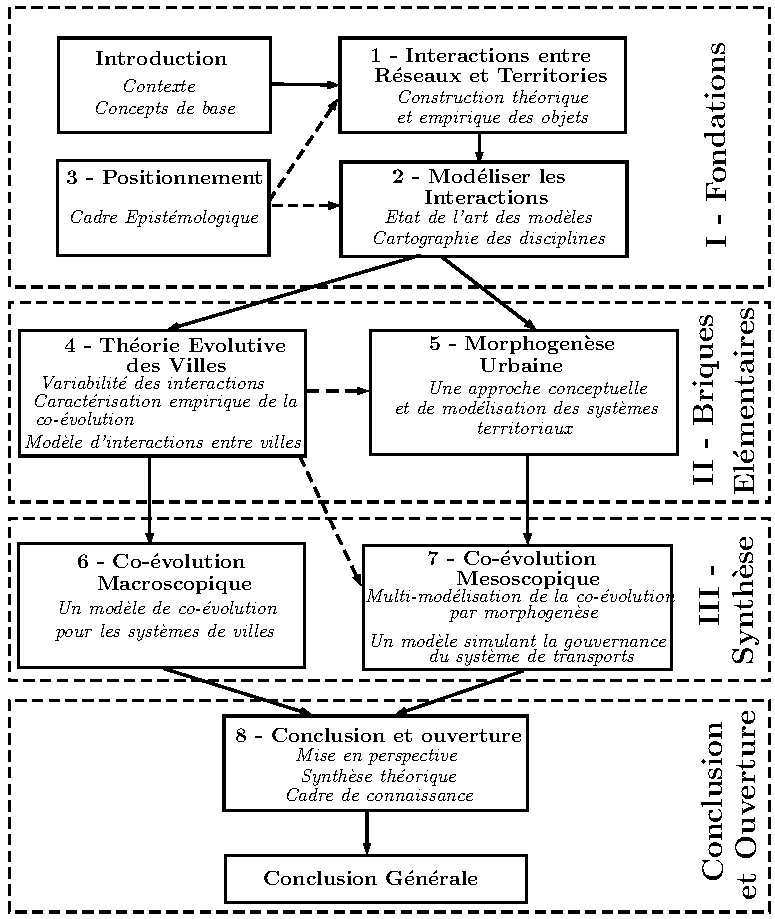
\includegraphics[width=\linewidth]{Figures/Theory/plan.pdf}
		
		\medskip
		
		\framecaption{\textbf{General organisation of this memoire.}\label{frame:intro:organisation}}{ \textbf{Organisation générale du mémoire.} Les flèches pleines donnent une dépendance directe (enchainement logique ou extensions), les flèches pointillées une dépendance indirecte (réutilisation de données ou de méthodes).\label{frame:intro:organisation}}
	\end{mdframed}
\end{figure}
%%%%%%%%%%%

%  Le troisième chapitre irrigue l'ensemble des autres chapitres, nous ne gardons que les relations initiales.

% \comment[AB]{intro = beau boulot !}

%\comment[FL]{Introduction \cn{关}
%\begin{itemize}
	%\item c'est seulement p11 que tu parles pour la premiere fois du sujet. Avant c'est de l'epistemo : pas une introduction a la these, mais une discussion - tres utile - sur les champs scientifiques. Garde cette discussion mais commence par une vraie introduction.[non, prefere garder cette strategie]
	%\item fin OK $\rightarrow$ et à positionner avant la partie epistemo.
%\end{itemize}
%}




%\paragraph{On linear reading}{Sur la lecture linéaire}

%%%%%%%
%% -- ON HOLD -- (depends on reflexive analysis - last appendix)


%\comment{expliquer notre position sur la difficulté d'une présentation linéaire, au delà de faire la synthèse. // bon bouquins y arrivent ? y réfléchir. la métaphore narrative intro/cl parties sera ce squelette linéaire. les deux approches sont compatibles.}


%\bpar{
%Research question and precise objects are deliberately fuzzy for now, as we postulate that the construction of a problematic can not be dissociated from the production of a corresponding theory. Reciprocally, it makes no sense to ask questions out of the blue, on objects that have been only partially or rapidly defined. Our preliminary question to enter the subject, that we can obtain from concrete cases such as our introducing anecdote or from preliminary literature review, is the following :
%}{
%Dans tous les cas, nous postulons que la construction d'une problématique ne peut être dissociée de la production d'une théorie correspondante. De manière réciproque, il n'y a aucun sens à poser des questions sorties de nulle part, sur des objets qui ont été seulement partiellement ou brièvement définis. Notre question préliminaire pour entrer dans le sujet, qu'on peut obtenir à partir de cas concrets comme l'anecdote introductive ou la revue de littérature préliminaire, est la suivante :
%}









\stars



